\documentclass[12pt,a4paper,titlepage]{article}
\usepackage[utf8]{inputenc}

\usepackage[left=1.5cm,right=2cm,top=2cm,bottom=2cm]{geometry}
\usepackage{amsmath}
\usepackage{amssymb}
\usepackage{amsthm}
\usepackage{hyperref}
\usepackage{graphicx}
\usepackage[space]{grffile}

\usepackage{listings}
\lstset{language=Java}


\newcommand{\class}[1]{$\mathtt{#1}$}

\author{Jonathan Visbecq, Gaspard Férey}
\title{Projet d'INF 431 \\ - \\ Rapport}


\begin{document}
\maketitle

\section*{Introduction}

\section*{Classes annexes}

\subsection*{La lecture des fichiers}

\begin{figure}
	\label{fig:fileManagerPackage}
	\centering
	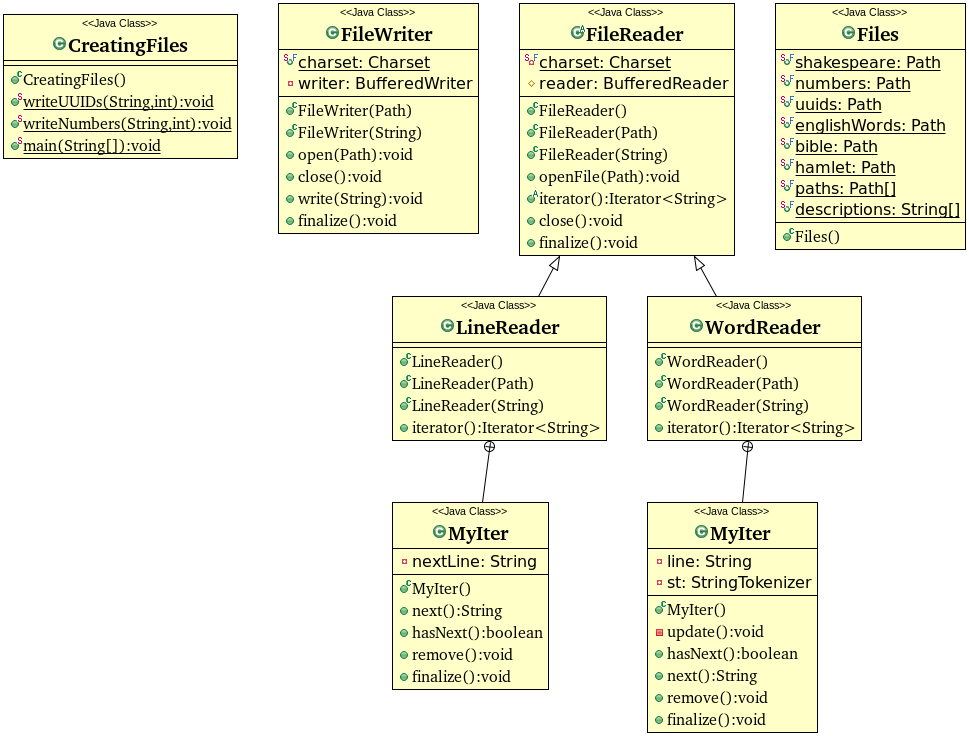
\includegraphics[scale=0.65, angle=90]{../Java Workspace/Test Hash/fileManagerPackage.png}
	\caption{Le package fileManagerPackage.}
\end{figure}

Le traitement du sujet suggère la manipulation fréquente de gros fichiers textes.\\
Les classes du package \class{FileManager} permettent de faciliter l'utilisation des fichiers. Par exemple, elles permettent de les désigner par leur chemin \class{Path} ou leur adresse \class{String} et gèrent les éventuelles exceptions lors du traitement en interne. En particulier, on y trouve :
\begin{itemize}
\item La classe abstraite \class{FileReader} qui permet d'ouvrir en lecture un fichier.\\
	Cette classe implémente l'interface \class{Iterable<String>} et permet donc de parcourir le fichier à l'aide d'une simple boucle \class{for}.
	Elle possède deux classes filles :
	\begin{itemize}
	\item La classe \class{WordReader} qui permet de lire un fichier mot à mot.
	\item La classe \class{LineReader} qui permet de lire un fichier ligne à ligne.
	\end{itemize}
\item La classe \class{FileWriter} qui permet l'écriture dans un fichier.
\item La classe \class{Files} qui est simplement un catalogue des fichiers souvent utilisés.
\item La classe \class{CreatingFiles} qui contient des fonctions qui permettent des générer des fichiers volumineux de test. En particulier, ils génèrent :
	\begin{itemize}
	\item Un fichier des nombres de 0 à n.
	\item Un fichier de n identifiants UUID générés pas Java.
	\end{itemize}
\end{itemize}

\subsection*{L'arithmétique en Java}
La classe \class{UnsignedArithmetic} du package \class{drafts} fournit des fonctions qui permettent la correcte implantation des opérateurs somme et minimum de deux entiers. En effet, Java utilise une implantation interne du type \class{int} qui tend à préserver le bit de signe (bit de poids le plus fort) lors de certaines opérations.

\subsection*{Communiquer}
La classe \class{Draft} du package \class{drafts} fournit, elle, des fonctions utiles à l'interface avec l'utilisateur. En particulier elle contient des méthodes d'affichage et d'utilisation de la console.




\newpage
\section{Le hachage}

\begin{figure}
	\label{fig:hashPackage}
	\centering
	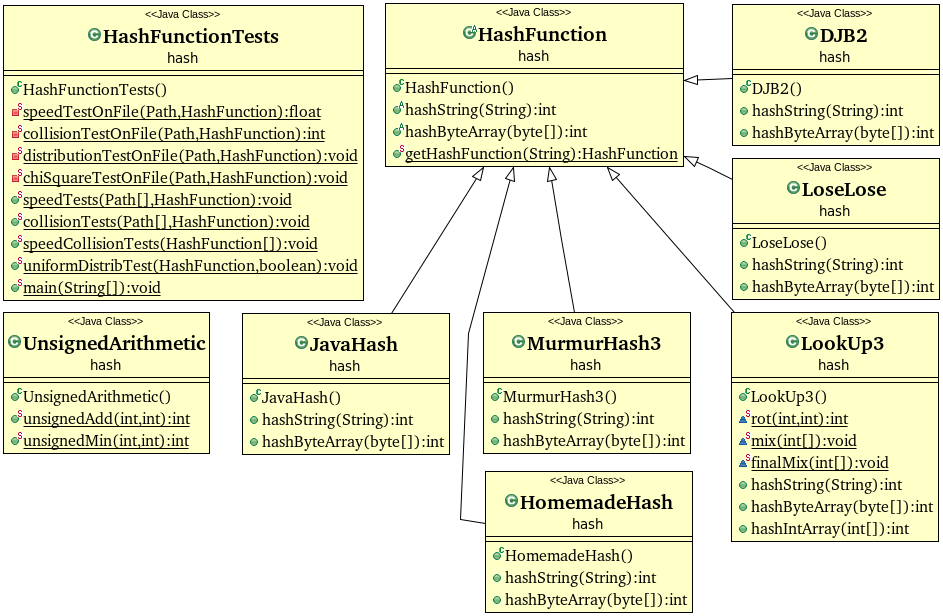
\includegraphics[scale=0.75, angle=90]{../Java Workspace/Test Hash/hashPackage.png}
	\caption{Le package hashPackage.}
\end{figure}

Nous avons choisit de définir chacune des fonctions de hachage comme des sous-classes de la classe abstraite \class{HashFunction}.
Ainsi cette classe impose la définition des méthodes suivantes :
\begin{lstlisting}
	public int hashByteArray(byte[] array);
	public int hashString(String s);
\end{lstlisting}
dont l'implémentation dépends, bien sur, de la fonction de hachage et qui implémentent le hachage des types de données qui nous intéressent.

\subsection{Le hachage \class{LookUp3}}
Cette classe implante un hachage tel qu'il est décrit à adresse \href{http://www.burtleburtle.net/bob/c/lookup3.c}{cette adresse}.

\subsection{Le hachage \class{MurmurHash3}}
Cette classe implante un hachage tel qu'il est décrit à adresse \href{http://en.wikipedia.org/wiki/MurmurHash}{cette adresse}.

\subsection{Autres hachages}
Principalement pour les comparer aux deux précédents, nous avons définit d'autres fonctions de hachage moins efficaces :
\begin{itemize}
\item \class{DJB2} dont la description peut être trouvée à \href{http://www.cse.yorku.ca/~oz/hash.html}{cette adresse}.
\item \class{JavaHash}, la fonction de hachage par défaut de Java.
\item \class{LoseLose}, dont la description peut être trouvée à \href{http://www.cse.yorku.ca/~oz/hash.html}{cette adresse}.
\item \class{HomemadeHash} 
\end{itemize}

\subsection{La classe \class{HashFunctionTests}}
Cette classe regroupe les méthodes permettant de comparer et tester les différentes fonctions de hachages.
On y trouve en particulier les méthodes suivantes :
\begin{itemize}

\item \begin{lstlisting}
private static float speedTestOnFile(Path path, HashFunction func)
\end{lstlisting}
Cette fonction parcours le fichier désigné par \class{path} et applique la fonction de hachage \class{func} sur chacun de ses mots. Elle retourne le temps que ce parcours a nécessité (en secondes).

\item \begin{lstlisting}
public static void speedTests(Path[] paths, HashFunction func)
\end{lstlisting}
Cette fonction effectue le même test sur tout les fichiers de \class{paths} et affiche les résultats dans la sortie standard.

\item \begin{lstlisting}
private static int collisionTestOnFile(Path path, HashFunction func)
\end{lstlisting}

\item \begin{lstlisting}
public static void collisionTests(Path[] paths, HashFunction func)
\end{lstlisting}
Cette fonction effectue le même test sur tout les fichiers de \class{paths} et affiche les résultats dans la sortie standard.

\item \begin{lstlisting}
private static void distributionTestOnFile(Path path, HashFunction func)
\end{lstlisting}

\item \begin{lstlisting}
private static void chiSquareTestOnFile(Path path, HashFunction func)
\end{lstlisting}

\end{itemize}



\newpage
\section{L'algorithme HyperLogLog}
La classe \class{HyperLogLog} contient les fonctions traitant la partie 2 du projet.\\
Les valeurs de $\alpha$ sont tabulées dans 
\begin{lstlisting}
static double[] alpha = { 0, 0.351194, 0.532435, 0.625609, ... };
\end{lstlisting}
Remarque : \class{alpha[b]} correspond à $\alpha_m$ avec $m=2^b$.\\

La fonction $\rho$ est déjà implantée en Java dans le package \class{Integer} ou elle porte le nom de \class{numberOfTrailingZeros}.
Nous fournissons également notre propre implantation :
\begin{lstlisting}
public static int rho(long x)
\end{lstlisting}



\newpage
\section{Similarités entre ensembles de données}





\newpage
\section{Fenêtre glissante}





\newpage
\section{Échantillonnage}





\newpage
\section{Souris}






\newpage
\section{Icebergs}





\newpage
\section*{Conclusion}




\end{document}
